\chapter{Abastecimento}
\label{abastecimento}

\par No presente trabalho, o sistema de abastecimento é todo o conjunto que engloba o sistema de alimentação e os processos necessários para que o oxidante líquido seja transferido para o foguete de forma remota, segura e no momento indicado pelo usuário. Pode-se ainda citar os processos ocorridos para a ignição como apresentado em \ref{sec:ignição}. 

\section{Fluxo de trabalho}

\par A seguir é apresentado um fluxograma do sistema de alimentação, figura \ref{fig:sistema de alimentacao}. Logo em seguida é caracterizado os componentes do sistema, desde os pré estabelecidos pelo cliente, até os definidos pelo grupo.

\begin{figure}[H]
\centering
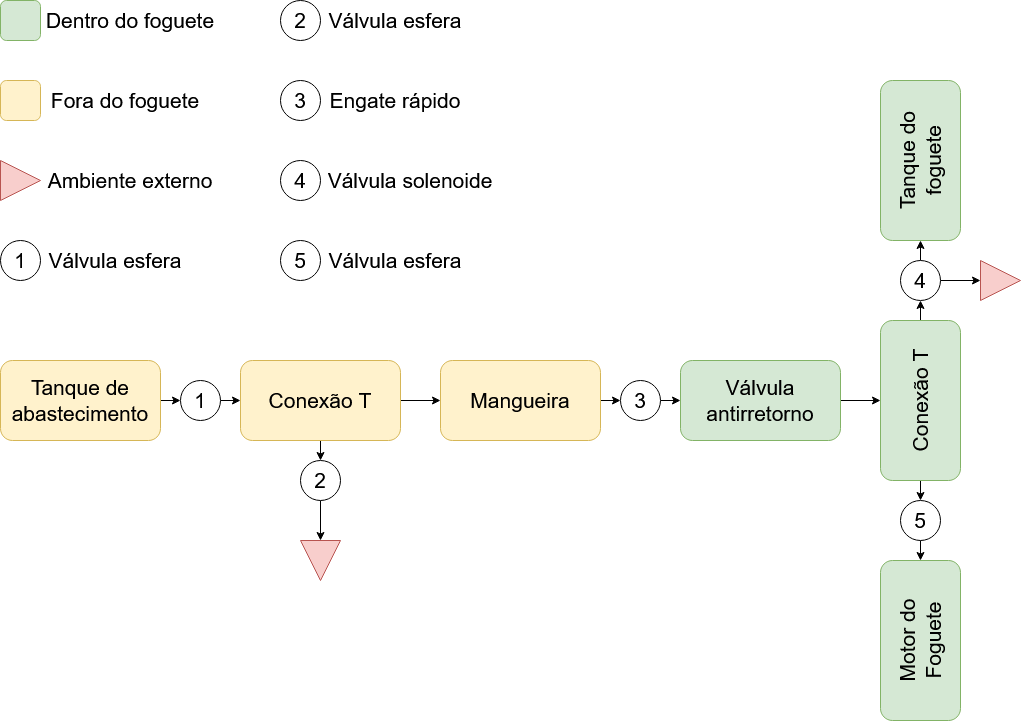
\includegraphics[width=0.9\textwidth]{figuras/diagramaAlimentacao}
\caption{Fluxograma do sistema de alimentação}
\label{fig:sistema de alimentacao}
\end{figure}


\par Com base no projeto desenvolvido pelo cliente \cite{capitalrocketteam2020}, o funcionamento do sistema de abastecimento ocorre em etapas, cada uma delas correspondendo ao estados das válvulas, se estão abertas ou fechadas conforme a ação desejada, figura \ref{fig:sistema de alimentacao}. 

\begin{enumerate}
    \item \textbf{Etapa 1 - Estado inicial}: todas as válvulas estarão fechadas, ou seja, o sistema estará em repouso, de modo a evitar qualquer vazamento antes do início do processo de abastecimento; 
    
    \item \textbf{Etapa 2 - Resfriamento do tanque do foguete}: abertura das válvulas 1 e 4, de modo a realizar a passagem de um fluxo inicial do fluido oxidante, com a finalidade de resfriar o tanque do foguete e otimizar seu abastecimento. O tempo de resfriamento fica a critério do usuário, e a etapa é encerrada com o fechamento das duas válvulas;
    
    \item \textbf{Etapa 3 - Abastecimento do tanque}: abertura da válvula 1, com posterior abertura e fechamento intermitente da válvula 4 para alívio da pressão interna do tanque do foguete durante seu abastecimento. O fluido oxidante é transportado, devido a fenômenos termodinâmicos, em estado de mistura (líquido e gás), e no tanque do foguete a sua fase gasosa deverá ser expulsa pela válvula 4, até o nível definido pelo usuário, este é controlado pela célula de carga que mede a variação de peso do foguete. Com base nos dados fornecidos pela célula de carga, o usuário avaliará se o tanque se encontra cheio, encerrando a etapa com o fechamento da válvula 1 e, caso aberta, da válvula 4; 
    \item \textbf{Etapa 4 - Alívio de pressão da mangueira}: abertura da válvula 2 para expurgo do fluido oxidante que se encontra no interior da mangueira, de modo a equalizar sua pressão interna com a pressão ambiente, de modo a ser possível realizar seu desacoplamento do foguete. A existência de uma válvula anti-retorno na linha de abastecimento impede que o fluido contido no tanque do foguete seja também expurgado nessa fase; 
    \item \textbf{Etapa 5 - Desacoplamento da mangueira}: acionamento do engate rápido, por meio de um atuador linear, de modo a desacoplar e afastar a mangueira do foguete. Essa etapa encerra o processo de abastecimento, e o foguete está preparado para o lançamento; 
    \item \textbf{Etapa 6 - Ignição do foguete}: após o acionamento do ignitor junto ao combustível no motor do foguete, por meio do comando da estação de controle, é feita a abertura da válvula 5, que injetará o fluido oxidante do tanque do foguete na câmara de combustão no interior do motor. Assim o encontro desse fluido com o combustível e o calor gerado pelo ignitor iniciará a combustão principal, e o foguete iniciará sua decolagem.
\end{enumerate}

\par Como mencionado, durante o transporte do fluido oxidante do tanque de abastecimento para o tanque do foguete, fenômenos termodinâmicos ocorrem, como a queda de temperatura provocada pela passagem do fluido conforme ele vai reduzindo a pressão à qual estava submetido no cilindro comercial (por volta de 50 bar). Em alguns casos, esse fenômeno é desejável, como para o resfriamento do tanque do foguete, em outros, ele pode apresentar um problema, como o congelamento de válvulas e atuadores que não estejam nas especificações adequadas. Do mesmo modo, a atuação das válvulas ocorrerá em situações em que o fluido estará a grande pressão, o que impede o manuseio delas manualmente, seja por necessidade, seja por questões de segurança. Ademais, não é recomendado o uso de mangueiras muito longas para o abastecimento, devido à perda do fluido durante seu transporte.

\par A solução proposta é o acoplamento de dois atuadores rotativos nas válvulas 1 e 2, os quais receberão um comando remoto de abertura e fechamento a partir da estação de controle. Para tanto, será necessário tanto o dimensionamento das opções comerciais para atuadores, desde o torque gerado por cada um dos modelos até sua natureza – se eletrônico ou pneumático, quanto o desenvolvimento de uma estrutura de suporte e adaptação entre esses atuadores e as válvulas e conexões do sistema de alimentação, a qual também deverá observar as características (variação de temperatura e pressão) do processo der abastecimento.

\par Deve-se atentar ao fato de que o cliente pediu uma mudança de escopo onde ficou decidido que o dispositivo mecânico responsável pelo desacoplamento e remoção física da mangueira do foguete, a etapa 5 do sistema, representado por 3 na figura \ref{fig:sistema de alimentacao},  será desenvolvido por eles. Cabendo à equipe apenas desenvolver a solução responsável por enviar o comando de desengate a partir da estação de controle. Eles ainda demandaram que esse sistema será baseado em um servo motor ou um motor como usado pelo grupo na solução de válvulas.

\section{Caracterização dos componentes}

\par Nessa seção estão apresentadas as características especificas dos componentes do sistema de abastecimento.

\begin{itemize}

    \item \textbf{Tanque de abastecimento}: É um cilindro comercial fornecido pela empresa distribuidora de óxido nitroso. A válvula esfera, item 1 da figura \ref{fig:sistema de alimentacao}, deverá ser conectada no bocal de saída desse cilindro, com uso de adaptador caso necessário.
    \par Informações Técnicas: Cilindro de aço para 10 litros ou 7,0 Kg de óxido nitroso; Altura: 70 cm;    Diâmetro: 20 cm; Peso aproximado: 15 Kg.
    
    \item \textbf{Válvula esfera macho-fêmea 1/2 polegada NPT Flangeada}: É uma válvula de abertura de 90$^{\circ}$. Seu manipulo deverá ser retirado e a porca ligada à esfera de abertura/fechamento será conectada ao tarugo de conexão com o eixo do motor. 
     \par Informações Técnicas: figura \ref{valvula}.
    
    \item \textbf{Conector em T macho-fêmea-macho 1/2 polegada NPT}: São adaptadores em pontos de bifurcação do sistema hidráulico.
    \par Informações Técnicas: para conexões pneumáticas os Tee e cotovelos são forjados em latão, Liga UNS - C37700 - TM, que proporcionam maior dureza e resistência contra golpes, choques mecênicos e vibrações, com absoluta inexistência de porosidade e trincas. A pressão de trabalho precisa ser compatível com as especificações do tubo utilizado.
    
    \item \textbf{Tubo flexível 1/2 polegada de aço inox com tramas de aço}: É necessário por não reagir com o óxido nitroso, como ocorre com a borracha, comum nas mangueiras convencionais.
    
    \item \textbf{Engate rápido 3/4 polegada NPT}: É uma conexão composta por duas peças (macho e fêmea) e um anel de segurança. Somente movendo o anel é que as duas peças podem ser desconectadas.
    
    \item \textbf{Válvula anti-retorno macho-fêmea 3/4 polegada NPT}: É uma válvula de sentido único, ligada ao engate rápido da mangueira e o conector T que liga o tanque ao motor dentro do foguete. Evita que o óxido nitroso volte no sentido do tanque de abastecimento.
    
\end{itemize}   

 
\par No anexo \ref{ane:Elementos do sistema de alimentação} é apresentada mais informações técnicas de cada um dos elementos descritos nessa seção.

\section{Atuador}

\par O dimensionamento do atuador exige conhecimento do torque necessário para abrir a válvula esfera. Um estudo feito por Silva, aponta que o torque inicial necessário para abrir uma válvula esfera sob pressão de óxido nitroso é de 2 N.m.
\par Assim a solução para a abertura e fechamento de válvulas por comando remoto é a utilização de um motor de 12 Volts acoplado com um sistema de caixa redutora conectado a válvula. O sistema de caixa redutora possui a função de aumentar o torque do motor elétrico, diminuindo a velocidade de rotação.
\par A proposta é utilizar um motor de para-brisa que já possui uma caixa redutora acoplada a ele. 

\par O óxido nitroso se apresenta em uma mistura líquido-vapor, com pressão de aproximadamente 57 bar a temperatura ambiente de 25$^{\circ}$C. Admitindo uma margem de segurança, decidiu-se impor o critério de que a válvula deve suportar pressões de pelo menos 68 bar e temperaturas mínimas de até -20$^{\circ}$C. 

\par O atuador deve-se ter um torque mínimo que vai depender da válvula a ser utilizada, pode ser pesquisada o torque necessário para abrir a partir de dados do fabricante. No \textit{datasheet} da válvula escolhida é mostrado um torque de aproximadamente 1,5 N.m. e tempo de resposta de aproximadamente 2 segundos. Com base nesse torque, foram selecionadas duas opções
\par O Motor de vidro elétrico de carro: necessita ponte H (~R\$25) para realizar abertura e fechamento. Posição intermediária difícil de se obter, não há precisão na posição do motor. 
\par Informações técnicas: Voltagem 12V; Consumo 1,3A; Força 9,12 N.m / 93Kg.cm; Valor de ~ R\$60.

\par Servo motor Ds3218: consegue ajustar bem a posição, possui um maior controle de vazão. Consumo bem menor que o motor. É mais caro e gera menos torque, precisaria-se de dois servos para cada válvula, para trabalhar com segurança.
\par Informações técnicas: Voltagem 7.2 V; Consumo 100 mA; Força 2,19 N.m / 22.3 Kg.cm; Valor ~ R\$135

\par Assim, a escolha do atuador permeia o subnúcleo de energia, pois os valores de corrente são bem diferentes. Além disso, é necessário delimitar o preço, pois na verdade há no mercado válvulas esferas com atuadores elétricos pronto para uso, entretanto, como a pressão de trabalho é alta e a temperatura é baixa, o fluido no nosso projeto exige uma válvula robusta, que por sua vez exige um motor tão robusto quanto para abrir as válvulas, o custo de uma pronta é muito elevado de ~ R\$1000 cada. 

\par Com isso apresentado, a escolha foi do motor de vidro elétrico de carro que tem seus aspectos técnicos apresentados no anexo \ref{motorcarro}.

\subsection{Adaptador do atuador}
\label{subsec:atuador}
\par A descrição do adaptador do atuador é apresentada no manual de montagem no Apêndice \ref{Manual_de_montagem}. Na figura \ref{fig:adap} é possível vê como ficou o sistema.

\begin{figure}[H]
\centering
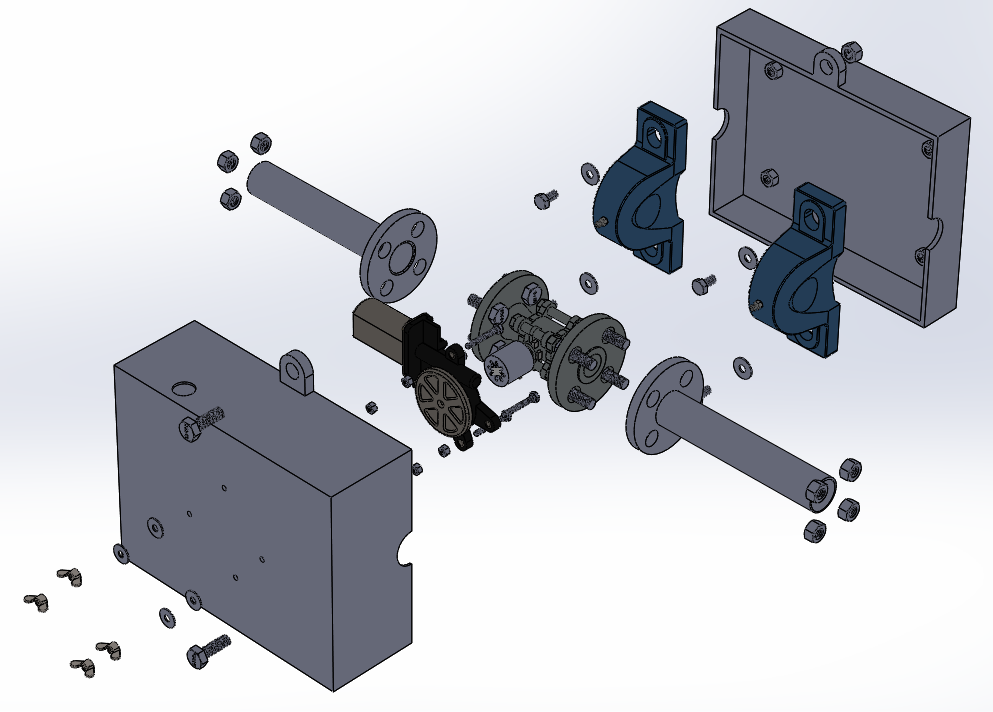
\includegraphics[width=0.9\textwidth]{figuras/explodida_valvula.png}
\caption{Vista explodidada do Adaptador}
\label{fig:adap}
\end{figure}


\section{Oxido Nitroso}
\label{sec:n2o}

A escolha do óxido nitroso como parte do par propelente é justificada pelas vantagens que esse gás industrial traz devido às suas características. Como já mencionado, esse gás é auto pressurizante, podendo ser armazenado a altas pressões (por volta de 50bar) a temperatura ambiente (20ºC), o que dispensa a necessidade de sistemas de pressurização e expulsão do tanque para o motor do foguete (necessitando apenas a abertura da válvula para o início da ignição). Além disso, é um gás comercial de fácil aquisição, relativamente barato em comparação a outros propelentes, é não tóxico, facilmente armazenável e de baixa inflamabilidade na ausência de seu par combustível \cite{rogerapazavasquez2017}. 

Abaixo algumas características físico-químicas importantes para o uso dessa substância \cite{rogerapazavasquez2017}: 

\begin{table}[H]
\centering
\begin{tabular}{|l|l|}
\hline
Massa molar & $44,013 kg/mol$ \\ \hline
Ponto de ebulição & $-88,5 ^{\circ}C$  \\ \hline
Ponto de fusão & $-90,8 ^{\circ}C$  \\ \hline
Temperatura crítica & $36,4 ^{\circ}C$ \\ \hline
Pressão crítica & $72,45 bar$  \\ \hline
Pressão de vapor (20 $^{\circ}$C) & $50,8 bar$  \\ \hline
Condutividade térmica (0 $^{\circ}$C) & $14,57 mW/(m.K)$  \\ \hline
Entalpia de formação & $82 kJ/mol$  \\ \hline
\end{tabular}
\caption{Características físico-químicas do óxido nitroso}
\label{tab:n2o}
\end{table}

\par Para fins do presente trabalho, a temperatura do gás é o parâmetro mais importante, uma vez que ela pode afetar o funcionamento do sistema de alimentação. Como dito, o óxido nitroso é armazenado à alta pressão e à temperatura ambiente. Isso significa que, quando é aberta a válvula do cilindro de abastecimento, ocorre uma queda de pressão do gás enquanto ele passa pelo sistema de alimentação, o que incorre numa queda de temperatura brusca, o cliente relatou que experiências passadas mostraram risco de congelamento de válvulas caso estas não fossem capazes de trabalhar a baixas temperaturas. 

%\section{Modelagem matemática}


\section{Simulação hidráulica}

\par Para a solução do nosso problema é necessária a criação de um adaptador para as válvulas do sistema de abastecimento. Esse sistema tem por objetivo transportar o propelente líquido do tanque de abastecimento para o tanque do foguete. Assim uma simulação que se aproxime do sistema eletromecânico desenvolvido, foi feita como meio de verificar sua usabilidade.

\subsection{Metodologia}

\par A simulação do sistema de abastecimento foi feita no software \textit{Simulink/Matlab} pois se trata de uma ferramenta confiável e conhecida no ramo de engenharia. A robustez do software se torna aliada uma vez que possui blocos nativos que representam fisicamente cada um dos componentes, permitindo uma maior agilidade na montagem e modelagem do problema. 

\par O projeto do sistema de alimentação foi desenvolvido usando-se o \textit{Simscape Fluids}, uma ferramenta do \textit{Matlab/Simulink}, onde ele fornece bibliotecas de componentes para modelagem e simulação de sistemas de fluidos, incluindo modelos de bombas hidráulicas, válvulas, atuadores, dutos e trocadores de calor. Para o abastecimento de combustível do foguete iremos usar o componentes de válvulas, atuadores e dutos integrado com as bibliotecas do \textit{Simscape Eletric}, um análogo a aquele para sistemas elétricos. 

\par O uso dessa ferramenta se da pois a mesma ajuda no desenvolvimento de sistemas de controle, onde é possível se testar o desempenho em nível de sistema. Com isso a principal biblioteca utilizada é a de Modelos Hidráulicos, na qual está-se presente os blocos hidráulicos básicos de temperatura constante seguindo-se as técnicas de modelagem apresentadas.

\par A seguir são apresentadas as etapas essenciais para construir e simular um modelo físico de sistema. A figura \ref{fig:metodologia} mostra o passo a passo para esse desenvolvimento.

\begin{figure}[h!]
\centering
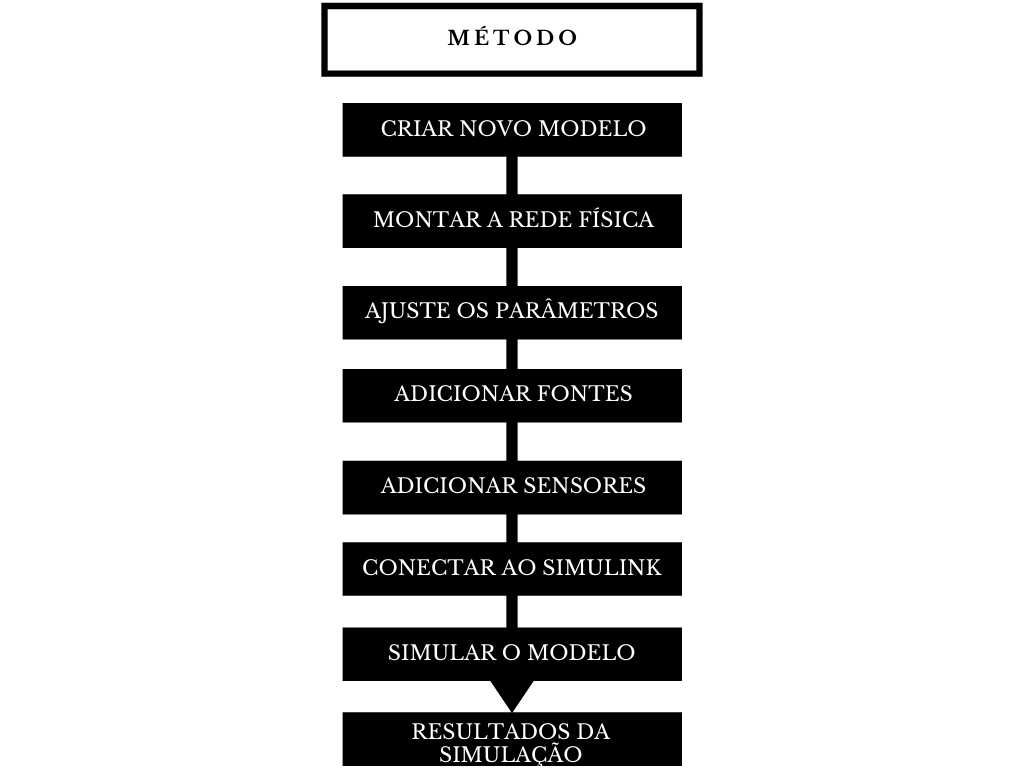
\includegraphics[width=0.9\textwidth]{figuras/metodo.png}
\caption{Etapas de simulação}
\label{fig:metodologia}
\end{figure}

\begin{enumerate}
    \item Etapa 1: Criar um novo modelo 
    \item Etapa 2: Montar a rede física, para modelar o sistema, adiciona-se blocos das bibliotecas \textit{Simscape} a um modelo e, em seguida, os conecta a uma rede física. 
    \item Etapa 3: Ajuste os parâmetros do bloco e as metas variáveis
    \item Etapa 4: Adicionar fontes, definir sinais de entrada.
    \item Etapa 5: Adicionar sensores, para medir as quantidades da rede física. 
    \item Etapa 6: Conectar ao \textit{Simulink} com blocos de interface
    \item Etapa 7: Simular o modelo
    \item Etapa 8: Ver os resultados da simulação
\end{enumerate}


\par A simulação matemática no ambiente do software foi ajustada com os parâmetros da tabela \ref{tab:abas} e os demais, por se tratarem de parâmetros que não alteram significativamente o resultado, foram deixados os valores padrão do programa.

\par Para as propriedades do fluído segue-se o que foi apresentado na seção \ref{sec:n2o}. Assim mesmo o óxido nitroso se apresentando como uma mistura líquido-vapor, com pressão de aproximadamente 57 bar a temperatura ambiente de 25\degree C \cite{Propriedades_termofisicas}, foi assumido que o escoamento do óxido nitroso se dá na fase líquida e a uma temperatura constante. Dado a complexidade de se fazer a modelagem e simulação como um escoamento em duas fases (líquido e vapor), como é o caso real. 

\begin{table}[H]
\centering
\begin{tabular}{|l|l|}
\hline
Densidade do óxido nitroso (a 25\degree C)              & 750 $kg/m^3$ \\ \hline
Viscosidade cinemática (líquido)            & $0,0639 x 10^6  m^2/s$ \\ \hline
Volume de óxido nitroso            & 7  $L$ \\ \hline
Diâmetro das tubulações                      & 2 $cm$ \\ \hline
\end{tabular}
\caption{Parâmetros da simulação de abastecimento}
\label{tab:abas}
\end{table}


\subsection{Blocos usados para o nosso sistema.}


    \subsubsection{ Caracterização do fluído combustível - \textit{Custom Hydraulic Fluid} }
    \par O primeiro passo é caracterizar o fluido combustível que devera ser transportado, deve-se atentar ao fato de que essas propriedades serão consideradas constantes durante o tempo de simulação. Para o nosso caso o cliente especifica o uso do oxido nitroso, por isso esse é o fluido que trabalharemos aqui, assim suas propriedades são apresentadas na seção \ref{sec:n2o}.
    \par Este bloco atribui propriedades de fluido para todos os componentes montados no \textit{loop}. 
    \par Os parâmetros utilizados são: densidade; viscosidade cinemática (líquido); módulo de compressibilidade, assim se o escoamento for incompressível; quantidade relativa de ar preso.
    \par As variáveis necessárias são: volume do fluido; nível do fluido.
    
    \subsubsection{ Tanque de abastecimento - \textit{Tank}}
    \par Cilindro comercial fornecido pela empresa distribuidora do óxido nitroso. A válvula esfera deverá ser conectada no bocal de saída desse cilindro, com uso de adaptador caso necessário. 
    \par O bloco do Simulink indicado possue um sinal de saída que indica o volume de fluido no tanque e um sinal de entrada que é a porta de conservação hidráulica associada à entrada do tanque. A perda de carga pode ser inserida por meio do valor de \textit{pipeline pressure loss coefficient}. 
    \par Tanque com pressão constante, leva em conta a mudança no nível do fluido e por isso é fornecida a área de seção transversal do tanque. 
    \par Os parâmetros necessários são: pressurização; nível do fluido; diâmetro da tubulação de entrada; coeficiente de perda de pressão do duto.
    
    \subsubsection{ Válvula esfera - \textit{Ball Valve} }
    \par Este bloco modela a redução de fluxo devido a uma válvula de esfera em uma rede hidráulica. Possui duas portas hidráulicas sendo uma associada a entrada e outra associada saída da válvula. Possui uma porta de entrada de sinal físico que indica o deslocamento capaz de alterar o fluxo do fluido que passa pela válvula. 
    \par Os parâmetros necessários são: diâmetro da esfera; diâmetro do orifício; coeficiente de descarga; \textit{leakage area}; área interna entre as entradas da válvula.
    \par As variáveis necessárias são: queda de pressão; quociente de vazão.
    
    \subsubsection{ Conexão T - \textit{T-junction} }
    \par O bloco representa uma junção em T que consiste em um trecho principal e uma ramificação que se une ao trecho principal em um ângulo especificado. A junção como uma resistência hidráulica é especificada por seis coeficientes de perda de pressão que caracterizam a relação pressão-vazão para cada conexão possível para o fluxo direto e reverso. O bloco apresenta três entradas/saídas hidráulicas (A, B, A1) que representam o fluxo do fluido. 
    \par Os parâmetros de geometria da válvula são: diâmetro do tubo principal; diâmetro do tubo de ramificação; especificação de transição laminar; razão de pressão de fluxo laminar.
    \par A perda de pressão possui os seguintes coeficientes que podem ser alterados: coeficiente de perda de pressão AB; coeficiente de perda de pressão BA; coeficiente de perda de pressão A-A1; coeficiente de perda de pressão A1-A; coeficiente de perda de pressão A1-B; coeficiente de perda de pressão B-A1
    
    \subsubsection{ Ambiente externo - \textit{Hydraulic Reference}} \par O bloco de referência hidráulica representa uma conexão com a pressão atmosférica. O bloco possui apenas uma porta de conservação hidráulica.
    
    \subsubsection{ Mangueira - \textit{segmented Pipeline}}
	\par Este bloco representa a perda de pressão do fluido em tubulações hidráulicas com seções transversais circulares como um conjunto de segmentos de tubos idênticos, conectados em série. Cada segmento de tubo leva em consideração as propriedades resistivas, de inércia de fluido e compressibilidade de fluido. Possui duas portas hidráulicas sendo uma associada ao fluxo de entrada e outra associada ao fluxo de saída da tubulação. 
	\par Os parâmetros necessários são: diâmetro interno do tubo; comprimento do tubo; número de segmentos; comprimento equivalente agregado de resistências locais; altura de rugosidade da superfície interna; margem superior do fluxo laminar; margem inferior do fluxo turbulento; tipo de parede de tubo; coeficiente de pressão estática de diâmetro; constante de tempo do processo viscoelástico; relação de calor específico; pressões iniciais nos nós do modelo; pressão inicial; vetor de pressão inicial; taxa de fluxo inicial.
	
	\subsubsection{ Válvula anti-retorno - \textit{Check Valve}}
	\par Este bloco representa uma válvula de retenção hidráulica com o objetivo de permitir o fluxo em uma direção e bloqueá-lo na direção oposta. A válvula permanece fechada enquanto a diferença de pressão através da válvula é inferior à pressão de abertura da válvula. Quando a pressão de abertura é atingida, o membro de controle de fluxo é forçado a sair de sua sede, criando assim uma passagem entre a entrada e a saída. Se vazão e pressão forem altas o suficiente, a área é aumentada ainda mais até que o membro de controle alcance sua máxima abertura. Possui duas portas hidráulicas sendo uma associada ao fluxo de entrada e outra associada ao fluxo de saída da válvula. 
	\par Os parâmetros necessários são: área máxima de passagem; pressão de fissura; pressão máxima de abertura; coeficiente de vazão; especificação de transição laminar; razão de pressão de fluxo laminar; número crítico de Reynolds; área de vazamento; dinâmica de abertura; constante de tempo de abertura; área inicial;

\subsection{Resultados}

\begin{figure}[H]
\centering
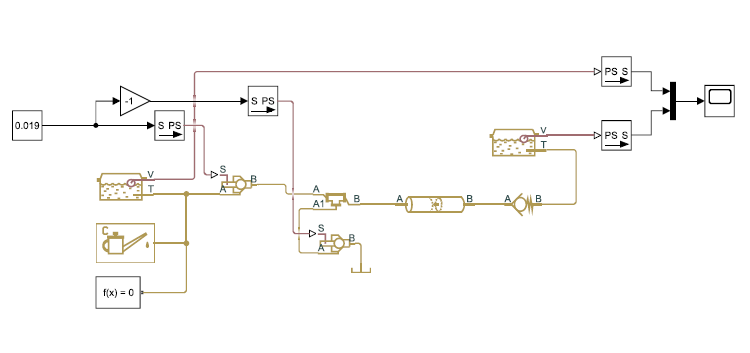
\includegraphics[width=1\textwidth]{figuras/diagrama_hidraulico.png}
\caption{Diagrama hidráulico}
\label{fig:metodologia}
\end{figure}

\begin{figure}[H]
\centering
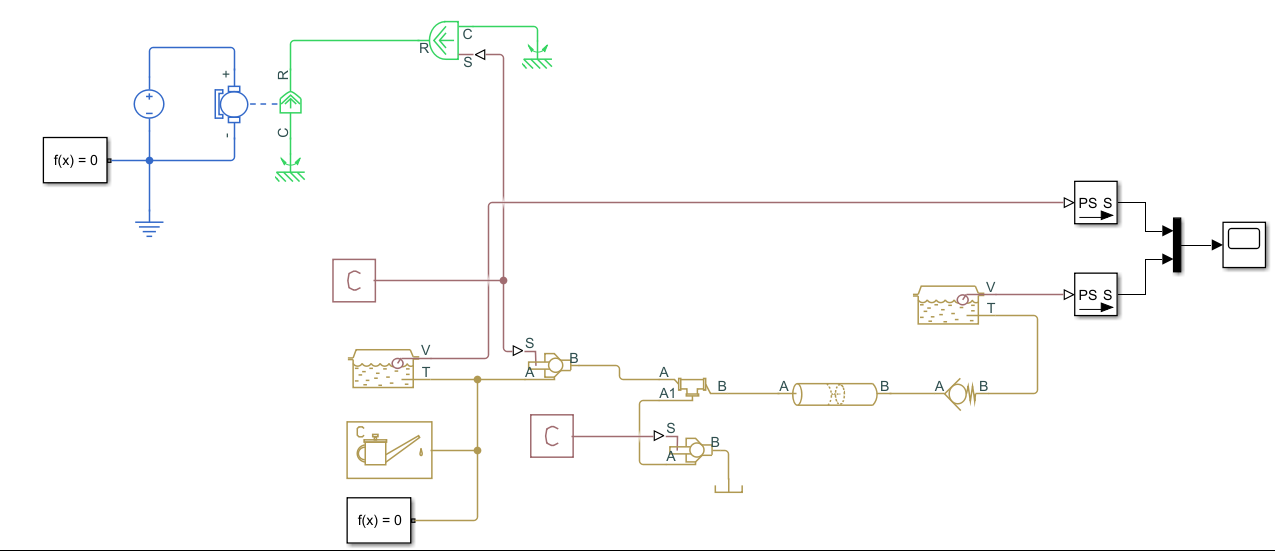
\includegraphics[width=1\textwidth]{figuras/diagrama_mecanico.png}
\caption{Diagrama eletromecânico}
\label{fig:metodologia}
\end{figure}

